\begin{figure}[htbp]
	\centering
	\usetikzlibrary{arrows.meta,calc,decorations.markings,angles,quotes}
	% --- proiezione obliqua: (x=profondita', y=oriz, z=vert) -> schermo ---
	\def\ax{0.5}\def\ay{0.30}
	\newcommand{\xyz}[3]{{#2 + (#1)*\ax},{#3 + (#1)*\ay}}
	\tikzset{midarrow/.style={postaction={decorate},decoration={markings, mark=at position 0.56 with {\arrow{Stealth}}}}}
	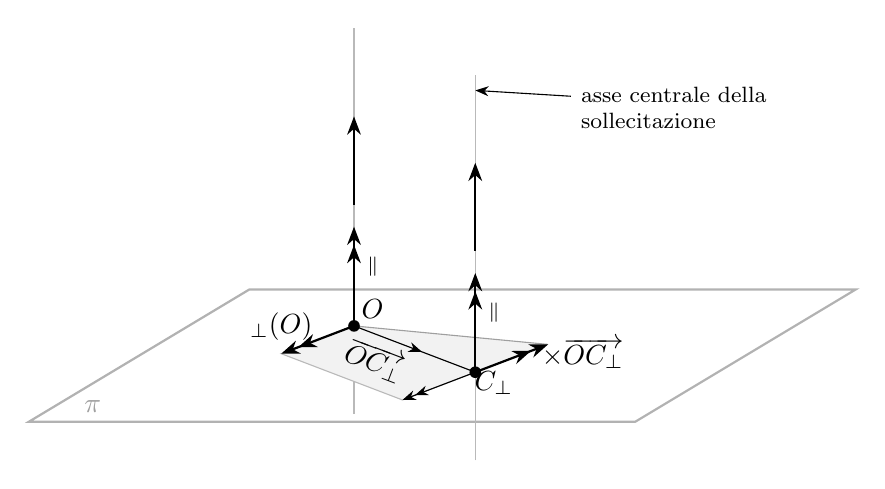
\begin{tikzpicture}[scale=1.4, >=Stealth, line width=0.8pt]
		
		%==== coordinate 3D (x=profondita', y=oriz, z=vert) ====
		\coordinate (Pi1) at (\xyz{-1.3}{-1.0}{0});   % era {-1.3}{-0.7}
		\coordinate (Pi2) at (\xyz{-1.3}{ 4.5}{0});   % era {-1.3}{ 3.5}
		\coordinate (Pi3) at (\xyz{ 2.7}{ 4.5}{0});   % era { 2.7}{ 3.5}
		\coordinate (Pi4) at (\xyz{ 2.7}{-1.0}{0});   % era { 2.7}{ 3.5}→ refuso: era { 2.7}{ 3.5}
		
		% O e suo asse
		\coordinate (O)     at (\xyz{1.6}{0.5}{0});
		\coordinate (Otop)  at (\xyz{1.6}{0.5}{2.7});
		\coordinate (Obot)  at (\xyz{1.6}{0.5}{-0.8});
		\coordinate (ThOa)  at (\xyz{1.6}{0.5}{1.10});
		\coordinate (ThOb)  at (\xyz{1.6}{0.5}{1.90});
		\coordinate (curlO) at (\xyz{1.6}{0.5}{2.12});
		\coordinate (uparO) at (\xyz{1.6}{0.5}{0.90});
		
		% u_perp(O): ora verso il BASSO-SINISTRA
		\coordinate (uperpO) at (\xyz{0.76}{0.26}{0});  % era {0.2}{0.1}
		
		% P_pi davanti-destra (OP_pi va in basso-destra): base 0.2,2.3 (era 1.886,2.5)
		\coordinate (Ppi)   at (\xyz{0.2}{2.3}{0});
		\coordinate (Ctop)  at (\xyz{0.2}{2.3}{2.7});
		\coordinate (Cbot)  at (\xyz{0.2}{2.3}{-0.8});
		\coordinate (ThCa)  at (\xyz{0.2}{2.3}{1.10});
		\coordinate (ThCb)  at (\xyz{0.2}{2.3}{1.90});
		\coordinate (curlC) at (\xyz{0.2}{2.3}{2.12});
		\coordinate (uparC) at (\xyz{0.2}{2.3}{0.90});
		
		% prodotto vettoriale = -u_perp(O): ora verso l'ALTO-DESTRA
		\coordinate (cross)  at (\xyz{1.04}{2.54}{0});  % era {1.6}{2.7}
		\coordinate (Bpar) at (\xyz{-0.64}{2.06}{0});
		
		
		%==== piano pi ====
		\draw[gray!60] (Pi1) -- (Pi2) -- (Pi3) -- (Pi4) -- cycle;
		\node[gray!75] at ($(Pi1)+(0.58,0.14)$) {$\pi$};
		
		%==== assi verticali ====
		\draw[gray!55, thin] (Obot) -- (Otop);
		\draw[gray!55, thin] (Cbot) -- (Ctop);
		
		%==== parallelogramma di lati u_perp(O) e OP_pi (evidenziato) ====
		\filldraw[gray!10, draw=gray!55, thin]	(O) -- (uperpO) -- (Bpar) -- (Ppi) -- cycle;
		
		%==== triangolo O--C_perp--(f x OC_perp) ====
		\fill[gray!10] (O) -- (Ppi) -- (cross) -- cycle;
		
		% u_perp(O) traslato in P_pi: opposto e collineare al prodotto vettoriale
		\draw[->>,  thin] (Ppi) -- (Bpar);
		%\node[font=\small, below=4pt, right] at (Bpar) {$\ub_{\perp}(O)$};
		
		%==== segmento O--(punta di vartheta x OP_pi) e ampiezza di rotazione vartheta ====
		\draw[draw=gray!75, thin] (O) -- (cross);
		%\pic[draw=black, ->, thin, angle radius=10mm, angle eccentricity=1.25,	"$\vartheta$"{font=\small, inner sep=1pt}] {angle = Ppi--O--cross};
		
		%==== vettori rotazione assiali + riccioli (sopra la doppia freccia) ====
		\draw[->, thick] (ThOa) -- (ThOb) node[right=1pt] {$\rb$};
		\draw[->, thick] (ThCa) -- (ThCb) node[right=1pt] {$\rb$};
		
		%==== costruzione nel piano ====
		%\draw[->, thin] (O) -- (Ppi);
		%\draw[midarrow, thin] (O) -- (Ppi);   % era  \draw[->, thin] (O) -- (Ppi);
		%\node[font=\small, below=1pt] at ($(O)!0.30!(Ppi)$) {$\overrightarrow{OC_\perp}$};   % era 0.55, below=2pt
		
		\draw[midarrow,thin] (O) -- (Ppi) node[midway, sloped, below,xshift=-12pt] {$\overrightarrow{OC_\perp}$};
		
		
		\draw[->>, thick] (O) -- (uperpO);
		\node[above=1pt] at (uperpO) {$\bm{\upmu}_{\perp}(O)$};
		\draw[->>, thick] (O) -- (uparO);
		\node[right=1pt] at ($(O)!0.6!(uparO)$) {$\bm{\upmu}_{\parallel}$};
		
		%==== a P_pi ====
		\draw[->>, thick] (Ppi) -- (uparC);
		\node[right=1pt] at ($(Ppi)!0.6!(uparC)$) {$\bm{\upmu}_{\parallel}$};
		\draw[->>, thick] (Ppi) -- (cross);
		\node[below right=-6pt] at (cross) {$\rb\times\overrightarrow{OC_\perp}$};
		
		
		
		%==== punti ====
		\fill (O)   circle (1.5pt) node[above right=-1pt] {$O$};
		\fill (Ppi) circle (1.5pt) node[below right=-4pt] {$C_\perp$};
		
		%==== annotazione asse centrale ====
		\node[align=left, font=\footnotesize] (lab) at ($(Ctop)+(1.8,-0.3)$)	{asse centrale della\\ sollecitazione};
		\draw[->, thin] ($(lab.north west)+(0,-0.18)$) -- ($(Ctop)!0.18!(ThCb)$);
		
	\end{tikzpicture}%
	\caption{Costruzione geometrica dell'asse centrale del
		sistema di forze. Il momento rispetto a $O$ si decompone
		nella componente $\bm{\upmu}^O_{\parallel}$, parallela a
		$\rb$ e invariante per tutti i poli, e nella componente
		$\bm{\upmu}^O_{\perp}$, giacente nel piano $\pi$
		ortogonale a $\rb$. Il punto $C_\perp$, intersezione
		dell'asse centrale con $\pi$, è determinato dalla
		condizione $\rb \times \protect\overrightarrow{OC_\perp}
		= -\bm{\upmu}^O_{\perp}$; l'asse centrale è la retta
		per $C_\perp$ parallela a $\rb$.}
	\label{f:asse_centrale_forze}
\end{figure}
